\documentclass[a4paper,11pt]{article}

\usepackage{fullpage} % Package to use full page
\usepackage{parskip} % Package to tweak paragraph skipping
\usepackage{amsmath}
\usepackage{hyperref}
\usepackage{amsmath,amsfonts,amsthm} % Math packages
\usepackage{graphicx}
\usepackage{listings}
\usepackage{caption}
\usepackage{subcaption}
\usepackage{color}
\usepackage{float}
\definecolor{codegreen}{rgb}{0,0.6,0}
\definecolor{codegray}{rgb}{0.5,0.5,0.5}
\definecolor{codepurple}{rgb}{0.58,0,0.82}
\definecolor{backcolour}{rgb}{0.95,0.95,0.92}
\definecolor{brown}{rgb}{0.59, 0.29, 0.0}
\definecolor{beaublue}{rgb}{0.74, 0.83, 0.9}
\definecolor{orange}{rgb}{1.0, 0.5, 0.0}
\definecolor{darkslategray}{rgb}{0.18, 0.31, 0.31}
\def\Xint#1{\mathchoice
	{\XXint\displaystyle\textstyle{#1}}%
	{\XXint\textstyle\scriptstyle{#1}}%
	{\XXint\scriptstyle\scriptscriptstyle{#1}}%
	{\XXint\scriptscriptstyle\scriptscriptstyle{#1}}%
	\!\int}
\def\XXint#1#2#3{{\setbox0=\hbox{$#1{#2#3}{\int}$}
		\vcenter{\hbox{$#2#3$}}\kern-.5\wd0}}
\def\dashint{\Xint-}

% Swap the definition of \abs* and \norm*, so that \abs
% and \norm resizes the size of the brackets, and the 
% starred version does not.
\makeatletter
\let\oldabs\abs
\def\abs{\@ifstar{\oldabs}{\oldabs*}}
%
\let\oldnorm\norm
\def\norm{\@ifstar{\oldnorm}{\oldnorm*}}
\makeatother
\definecolor{keywords}{RGB}{255,0,90}
\definecolor{comments}{RGB}{0,0,113}
\definecolor{red}{RGB}{160,0,0}
\definecolor{green}{RGB}{0,150,0}
\definecolor{codegreen}{rgb}{0,0.6,0}
\definecolor{codegray}{rgb}{0.5,0.5,0.5}
\definecolor{codepurple}{rgb}{0.58,0,0.82}
\definecolor{backcolour}{rgb}{0.95,0.95,0.92}
\definecolor{brown}{rgb}{0.59, 0.29, 0.0}
\definecolor{beaublue}{rgb}{0.74, 0.83, 0.9}
\definecolor{orange}{rgb}{1.0, 0.5, 0.0}
\definecolor{darkslategray}{rgb}{0.18, 0.31, 0.31}
\definecolor{deepblue}{rgb}{0,0,0.5}
\definecolor{deepred}{rgb}{0.6,0,0}
\definecolor{deepgreen}{rgb}{0,0.5,0}
\lstdefinestyle{myMatlabstyle}{
	language=Matlab,
	backgroundcolor=\color{white},   
	commentstyle=\color{codegreen},
	keywordstyle=\color{blue},
	identifierstyle=\color{brown},
	numberstyle=\tiny\color{codegray},
	stringstyle=\color{orange},
	basicstyle=\footnotesize,
	breakatwhitespace=false,         
	breaklines=true,                 
	captionpos=b,                    
	keepspaces=true,                 
	numbers=left,                    
	numbersep=5pt,                  
	showspaces=false,                
	showstringspaces=false,
	showtabs=false,                  
	tabsize=2
}
\lstdefinestyle{myPythonstyle}{
	language=Python, 
	basicstyle=\ttfamily\small, 
	keywordstyle=\color{blue},
	commentstyle=\color{green},
	stringstyle=\color{red},
	showstringspaces=false,
	identifierstyle=\color{black},
}
\lstset{language=Matlab,frame=single}
\lstset{language=Python,frame=single}

\title{AMATH 575: Problem Set 4}
\author{Jithin D. George, No. 1622555}
%\date{23/11/16}
% matrix environment
\newenvironment{mat}{\left[ \begin{array}{ccccccccccccc}}{\end{array}\right]}
\newcommand\bcm{\begin{mat}}
	\newcommand\ecm{\end{mat}}

\begin{document}

\maketitle
\begin{enumerate}

	\item

	\begin{enumerate}
		\item
		The first iteration has 20 blocks in 27 positions. After n iterations, this is ${\frac{20}{27}}^n$. As n goes to infinity, this becomes zero.
		
		\item
		Let us look at epsilon as a series.
		\[\epsilon_n = \big(\frac{1}{3}\big)^n\]
		Here, in the first iteration, $\epsilon$ refers to the side length on one of the 27 cubes. We would need 20 blocks in the first iteration and $20^n$ in the following ones.
		\[ D= \lim_{n -> \infty } \frac{ln(N)}{ln({\frac{1}{\epsilon}}^n)} = \lim_{n -> \infty } \frac{ln(20^n)}{ln({3}^n)} = \frac{20}{3}\] 
		\item
		For a d-dimensional hypercube, it would be divided by into $3^d$ boxes with edge length $\frac{1}{3}$.
		Of these, one box is deleted at each d-1 face and one central box is deleted as well. There are 2d d-1 faces.
	Thus , the number of boxes is given by $3^d-2d-1$.
	
		  
\[ D= \lim_{n -> \infty } \frac{ln(N)}{ln({\frac{1}{\epsilon}}^n)} = \lim_{n -> \infty } \frac{ln((3^d-2d-1)^n)}{ln(3^n)} =\frac{ln(3^d-2d-1)}{ln(3)}\] 
For 4-d, we get the dimension as 3.89

	\end{enumerate}	
	 
\item
The standard map requires around 7 iterations to see good horseshoes. We get the following result.
	\begin{figure}[H]
		\centering
		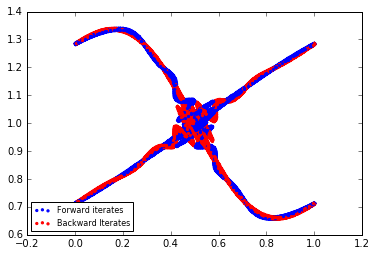
\includegraphics[width=10cm]{stahorse}
		\caption{Forward and backward iterations with the standard map }
	\end{figure}
Zooming in near the fixed point reveals horseshoes. The rectangle bounds one horseshoe quite well.
	\begin{figure}[H]
		\centering
		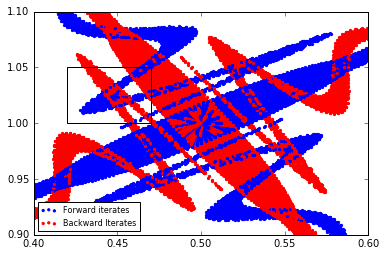
\includegraphics[width=10cm]{standardhorse}
		\caption{Horseshoes in the standard map }
	\end{figure}
\item
The following code generates the visualization of the horseshoe in the Henon map.
	\begin{lstlisting}[style=MyPythonstyle]
import numpy as np
import matplotlib.pyplot as plt
import decimal
decimal.getcontext().prec = 50

def hmap1(x):
	return [5-0.3*x[1]-x[0]**2,x[0]]
def hmap2(x):
	return [x[1],(5-x[0]-x[1]**2)/0.3] 

def plotstuff():
	xspace = np.linspace(-3,3,300)
	yspace = np.linspace(-3,3,300)
	for x in xspace:
		for y in yspace:
			[xnew,ynew]=hmap1([x,y])
			[xnew2,ynew2]=hmap2([x,y])
			plt.scatter(xnew,ynew,s=5,color='r')
			plt.scatter(xnew2,ynew2,s=5,color='b')
plt.show

plotstuff()   
	\end{lstlisting}
	\begin{figure}[H]
		\centering
		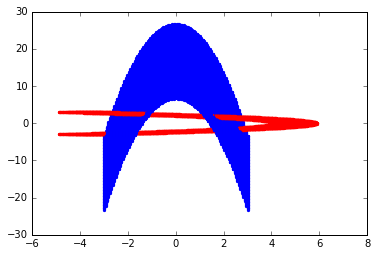
\includegraphics[width=10cm]{henonmap}
		\caption{Horseshoe in the Henon Map }
	\end{figure}
\item
We have
\[y'= Jy + F_2^R(y)+ F_3^R(y)+ \ldots+ F_{n+1}(y)+ O(n+2)\]
We use
\[y = z + h_{n+1}(z)\]
\[z' + Dh_{n+1}(z)z'= Jz + Jh_{n+1}(z) + F_2^R(z + h_{n+1}(z))+ F_3^R(z + h_{n+1}(z))+ \ldots+ F_{n+1}(y)+ O(n+2)\]
\[[I + Dh_{n+1}(z)]z'= Jz + Jh_{n+1}(z) + F_2^R(z + h_{n+1}(z))+  \ldots+ F_{n+1}(z + h_{n+1}(z))+ O(n+2)\]
\[z'= [I - Dh_{n+1}(z)](Jz + Jh_{n+1}(z) + F_2^R(z + h_{n+1}(z))+  \ldots+ F_{n+1}(z + h_{n+1}(z))+ O(n+2))\]
\[= Jz + Jh_{n+1}(z) -JzDh_{n+1}(z) + F_2^R(z)+\ldots + F_{n+1}(z)+ O(n+2))\]
	
\[= Jz + L^{n+1}(z) + F_2^R(z)+\ldots + F_{n+1}(z)+ O(n+2))\]
The operator is given by
\[ L^{n+1}(z) = Jh_{n+1}(z)-JDh_{n+1}(z)z  \]	
\item 
\[J = \bcm \lambda_1 &0 \\ 0 &\lambda2\ecm\]
We need to see the outputs of the operator L on the span of $H_2$ where L is given by
\[L h_2= Jh_2-Dh_2J\bcm x\\ y\ecm\]
Evaluating this would be much easier on a symbolic software. Instead of Mathematica, I use Sympy in Python. The code and output for the first case ($x^2$,0) are shown below.
	\begin{lstlisting}[style=MyPythonstyle]
from sympy import *
x= Symbol('x')
y= Symbol('y')
a= Symbol('a') #lambda1
b= Symbol('b') #lambda2
J= Matrix([[a,0], [0,b]])
H=Matrix([[x*2], [0]])
Dh=Matrix([[2*x,0], [0,0]])
L=J*H-Dh*J*Matrix([[x], [y]])
	\end{lstlisting}
	\begin{figure}[H]
		\centering
		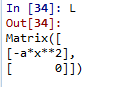
\includegraphics[width=5cm]{sympy}
		\caption{Output}
	\end{figure}
\[L\bcm x^2\\0 \ecm = \bcm -\lambda_1 x^2\\0 \ecm  \]
\[L\bcm y^2\\0 \ecm = \bcm (\lambda_1 -2\lambda_2) y^2\\0 \ecm  \]
\[L\bcm xy\\0\ecm = \bcm -\lambda_2 xy\\0 \ecm  \]
\[L\bcm 0\\xy\ecm = \bcm  0\\-\lambda_1xy \ecm  \]
\[L\bcm 0\\y^2\ecm = \bcm  0\\-\lambda_2y^2 \ecm  \]
\[L\bcm 0\\x^2\ecm = \bcm  0\\(\lambda_2 -2\lambda_1) x^2 \ecm  \]
If $\lambda_2 -2\lambda_1=0$, the normal form is given by
\[   x'= \lambda_1 x+ O(3)\]
\[   y'= \lambda_2 y+ a_1 x^2+ O(3)\]
or if $\lambda_1 -2\lambda_2=0$, the normal form is given by
\[   x'= \lambda_1 x+a_1 y^2+ O(3)\]
\[   y'= \lambda_2 y+ O(3)\]
Otherwise, the normal form is 
\[   x'= \lambda_1 x+ O(3)\]
\[   y'= \lambda_2 y+ O(3)\]
\item
\[L\bcm x^3\\0 \ecm = \bcm -2\lambda_1 x^3\\0 \ecm  \]
\[L\bcm y^3\\0 \ecm = \bcm (\lambda_1 -3\lambda_2) y^2\\0 \ecm  \]
\[L\bcm x^2y\\0\ecm = \bcm -(\lambda_1+\lambda_2)x^2y\\0 \ecm  \]
\[L\bcm xy^2\\0\ecm = \bcm -2\lambda_2 xy^2\\0 \ecm  \]
\[L\bcm 0\\x^2y\ecm = \bcm  0\\-2\lambda_1x^2y \ecm  \]
\[L\bcm 0\\xy^2\ecm = \bcm  0\\-(\lambda_1+\lambda_2)xy^2 \ecm  \]
\[L\bcm 0\\y^3\ecm = \bcm  0\\-2\lambda_2y^3 \ecm  \]
\[L\bcm 0\\x^3\ecm = \bcm  0\\(\lambda_2 -3\lambda_1) x^3 \ecm  \]
If $\lambda_2 -3\lambda_1=0$, the normal form is given by
\[   x'= \lambda_1 x+ O(4)\]
\[   y'= \lambda_2 y+ a_1 x^3+ O(4)\]
or if $\lambda_1 -3\lambda_2=0$, the normal form is given by
\[   x'= \lambda_1 x+a_1 y^3+ O(4)\]
\[   y'= \lambda_2 y+ O(4)\]
or if $\lambda_1 +\lambda_2=0$, the normal form is given by
\[   x'= \lambda_1 x+a_1 x^2y+ O(4)\]
\[   y'= \lambda_2 y+a_2 xy^2+ O(4)\]
Otherwise, the normal form has only the terms from second order and in the best case scenario becomes 
\[   x'= \lambda_1 x+ O(4)\]
\[   y'= \lambda_2 y+ O(4)\]
\item
Takens-Bogdanov has the following J.
\[J = \bcm 0 &1\\0&0\ecm\]
\[L\bcm x^3\\0 \ecm = \bcm -3x^2y\\0 \ecm  \]
\[L\bcm y^3\\0 \ecm = \bcm 0\\0 \ecm  \]
\[L\bcm x^2y\\0\ecm = \bcm -2xy^2\\0 \ecm  \]
\[L\bcm xy^2\\0\ecm = \bcm -y^3\\0 \ecm  \]
\[L\bcm 0\\x^2y\ecm = \bcm  x^2y\\-2xy^2 \ecm  \]
\[L\bcm 0\\xy^2\ecm = \bcm  xy^2\\-y^3 \ecm  \]
\[L\bcm 0\\y^3\ecm =  \bcm  y^3\\0 \ecm\]
\[L\bcm 0\\x^3\ecm =  \bcm  x^3\\-3x^2y \ecm  \]
We see that L cannot span $\bcm 0\\x^3\ecm$ and one of $\bcm x^3\\0\ecm$ and $\bcm 0\\-3x^2y\ecm$   
Thus,we get the normal form to be
\[   x'= y+ a_1x^2+ a_2x^3+O(4)\]
\[   y'= a_2x^2+ a_4x^3+a_5y^3+ O(4)\]

	\end{enumerate} 
\end{document}